\documentclass[12pt]{article}
\usepackage{graphicx}
\usepackage{geometry}
\usepackage{fancyhdr}
\usepackage{tabularx}
\usepackage{tikz}
\usetikzlibrary{arrows.meta, positioning}

\geometry{a4paper, margin=1in}
\pagestyle{fancy}
\fancyhf{}
\fancyhead[R]{Software Design Document}
\setlength{\headheight}{14.5pt}
\addtolength{\topmargin}{-2.5pt}

\title{
    {\Huge\textbf{Software Design Document}}\\[15mm]
    {\LARGE Sleep Fixer App}\\[15mm]
    {\Large Group 6}
}
\author{Dang Nguyen \quad Rafael Caldera \\ Yohei Oya \quad Yuanwei Chen\\[15mm]}
\date{December 2025}

\begin{document}

\maketitle
\newpage

\tableofcontents
\newpage

% ---------------------------------------------------------------
\section*{Revision History}
\addcontentsline{toc}{section}{Revision History}

\begin{table}[h!]
\centering
\begin{tabular}{|c|c|c|c|}
\hline
\textbf{User} & \textbf{Date} & \textbf{Reason for Changes} & \textbf{Version} \\
\hline
Dang Nguyen & 12/6/2025 & Added core app foundation  & 1.0 \\
\hline
Rafael Caldera & 4/6/2026 & Added notifications, streaks, weekly reports & 2.0 \\
\hline
Yohei Oya & 8/8/2026 & Added insights, community, journal, improved charts & 3.0 \\
\hline
Yuanwei Chen & 12/9/2026 & Added performance, accessibility, security, languages & 4.0 \\
\hline
\end{tabular}
\end{table}

\newpage

% ---------------------------------------------------------------
\section{Introduction}

\subsection{Purpose of This Document}
This Software Design Document (SDD) describes the design of the Sleep Fixer App across four snapshots of development. It explains how the system structure, core features, and user interface evolve over time. This document is written as a simplified, junior-college level mock SDD for practice.

\subsection{Intended Audience}
This SDD is intended for:
\begin{itemize}
    \item Developers implementing app features
    \item QA testers reviewing functionality
    \item Project team members who need a clear, organized overview of the design
\end{itemize}

\subsection{Overview of the System}
The Sleep Fixer App helps users improve sleeping habits through gradual bedtime adjustments.  
Key ideas include:
\begin{itemize}
    \item Users enter current and desired bedtime.
    \item App generates a day-by-day shift plan.
    \item User logs progress daily.
    \item The app provides notifications, insights, and streak tracking.
\end{itemize}

The system grows in features across **Snapshots 1–4**.

\newpage

% ---------------------------------------------------------------
\section{System Architecture}

\subsection{High-Level Workflow}
\begin{figure}[h!]
\centering
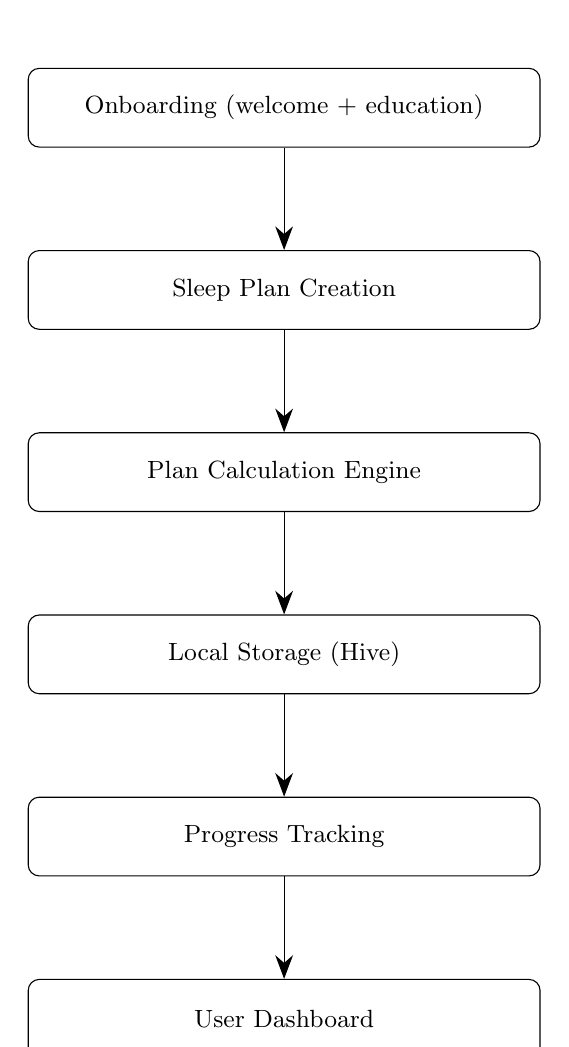
\begin{tikzpicture}[
    node distance=1.3cm,
    box/.style={
        rectangle, draw, rounded corners,
        minimum width=6.5cm, minimum height=1cm, align=center
    },
    >={Stealth[length=3mm]},
    every node/.style={font=\small}
]

\node[box] (onboarding) {Onboarding (welcome + education)};
\node[box, below=of onboarding] (plan) {Sleep Plan Creation};
\node[box, below=of plan] (engine) {Plan Calculation Engine};
\node[box, below=of engine] (storage) {Local Storage (Hive)};
\node[box, below=of storage] (tracking) {Progress Tracking};
\node[box, below=of tracking] (dash) {User Dashboard};

\draw[->] (onboarding) -- (plan);
\draw[->] (plan) -- (engine);
\draw[->] (engine) -- (storage);
\draw[->] (storage) -- (tracking);
\draw[->] (tracking) -- (dash);

\end{tikzpicture}
\caption{High-level system workflow (Snapshot 1 foundation)}
\end{figure}

The main flow of the app is:
\begin{enumerate}
    \item User completes onboarding.
    \item User enters bedtime information.
    \item App generates a personalized schedule.
    \item App saves the schedule and progress data.
    \item User records progress each day.
    \item Dashboard shows status, tips, streaks, or insights.
\end{enumerate}

\newpage

\subsection{Main Components}

\subsubsection{Presentation Layer (Flutter UI)}
\begin{itemize}
    \item \textbf{OnboardingScreen} – introduces app purpose.
    \item \textbf{PlanCreationScreen} – collects current + target bedtime.
    \item \textbf{FullPlanScreen} – displays daily targets.
    \item \textbf{ProgressTrackingDialog} – allows entering actual bedtime.
    \item \textbf{ProfileScreen} – shows summary and settings.
    \item \textbf{Notifications Panel} (Snapshot 2).
    \item \textbf{Journal Page} (Snapshot 3).
    \item \textbf{Community Page} (Snapshot 3).
    \item \textbf{Language + Accessibility Settings} (Snapshot 4).
\end{itemize}

\subsubsection{Business Logic Layer}
\begin{itemize}
    \item SleepPlanCalculator – determines shift size and plan length.
    \item ProgressTrackingService – evaluates bedtime accuracy and streaks.
    \item WeeklyReportGenerator (Snapshot 2).
    \item InsightsEngine (Snapshot 3).
    \item NotificationScheduler (Snapshot 2).
\end{itemize}

\subsubsection{Data Layer}
\begin{itemize}
    \item HiveService – local offline storage.
    \item FirebaseService – cloud backup + community features (Snapshot 3).
    \item SleepPlan Model – holds a user's schedule settings.
    \item SleepProgress Model – holds daily progress.
    \item JournalEntry Model (Snapshot 3).
    \item CommunityPost Model (Snapshot 3).
\end{itemize}

\newpage

% ---------------------------------------------------------------
\section{Core Design Details}

\subsection{Data Storage}

\textbf{Snapshot 1 – Local Database Only}
\begin{itemize}
    \item \textbf{sleep\_settings}: plan configuration.
    \item \textbf{sleep\_progress}: daily entries.
\end{itemize}

\textbf{Snapshot 3 – Cloud Storage Added}
\begin{itemize}
    \item Firebase stores:
    \begin{itemize}
        \item community posts
        \item cloud backups
        \item challenge participation
    \end{itemize}
\end{itemize}

\subsection{Example Progress Entry}
\begin{verbatim}
{
 "date": "2025-12-02",
 "targetTime": "22:00",
 "actualTime": "22:15",
 "status": "within30Min",
 "notes": "Felt good tonight"
}
\end{verbatim}

\subsection{Example Sleep Plan}
\begin{verbatim}
{
 "currentBedtime": "23:30",
 "goalBedtime": "22:00",
 "shiftSize": 20,
 "planLength": 9,
 "startDate": "2025-12-01"
}
\end{verbatim}

\subsection{Key Algorithms}

\subsubsection{Shift Size Calculation}
\begin{verbatim}
IF difference <= 60 min → 15-minute shift
ELSE IF <= 180 min → 20-minute shift
ELSE → 30-minute shift
\end{verbatim}

\subsubsection{Plan Duration}
\begin{verbatim}
shifts = CEILING(totalDifference / shiftSize)
daysPerShift = 1 or 2 depending on difficulty
totalDays = shifts × daysPerShift
\end{verbatim}

\subsubsection{Progress Status Rules}
\begin{verbatim}
0 minutes → onTarget
<= 30 min → within30Min
<= 60 min → within1Hour
> 60 min → offTarget
\end{verbatim}

\subsection{Additional Logic by Snapshot}

\subsubsection*{Snapshot 2 – Engagement Logic}
\begin{itemize}
    \item Notification reminders 30 minutes before bedtime.
    \item Morning check-in questions.
    \item Streak tracking increases motivation.
    \item Weekly report generator summarizes progress.
\end{itemize}

\subsubsection*{Snapshot 3 – Personalization Logic}
\begin{itemize}
    \item Insights identify user patterns (ex: “Fridays are harder”).
    \item Journal entries connect habits to sleep quality.
    \item Anonymous community sharing.
    \item Improved long-term charts and exportable reports.
\end{itemize}

\subsubsection*{Snapshot 4 – Stability and Security}
\begin{itemize}
    \item Faster loading and battery-efficient performance.
    \item Larger fonts, better contrast, screen reader support.
    \item Fingerprint / Face ID lock.
    \item Encrypted local data.
\end{itemize}


\newpage

% ---------------------------------------------------------------
\section{User Interface Design}

\subsection{Using the App}

\textbf{Snapshot 1 – Basic Flow}
\begin{enumerate}
    \item Onboarding screens introduce the concept.
    \item User enters current and desired bedtimes.
    \item App creates a gradual plan.
    \item User logs bedtime daily.
    \item Dashboard shows progress.
\end{enumerate}

\subsubsection*{Snapshot 2 – Added UI Features}
\begin{enumerate}
    \item Streak meter displayed under the daily goal.
    \item Notification settings page.
    \item Weekly report card on dashboard.
\end{enumerate}

\subsubsection*{Snapshot 3 – Added User Tools}
\begin{enumerate}
    \item Journal entry modal.
    \item Insights screen with personalized suggestions.
    \item Community challenge page.
    \item Expanded charts for weekly/monthly views.
\end{enumerate}

\subsubsection*{Snapshot 4 – Final UI Polish}
\begin{enumerate}
    \item Larger font mode.
    \item Multi-language selection (English, Spanish, French).
    \item Security settings panel (biometric lock).
    \item Smooth transitions and refined animations.
\end{enumerate}

\subsection{Navigation Layout}
\begin{itemize}
    \item \textbf{Home}: daily goals, progress, streaks
    \item \textbf{Insights}: personalized advice
    \item \textbf{Community}: achievements + challenges
    \item \textbf{Profile}: settings, language, privacy
\end{itemize}

\newpage

% ---------------------------------------------------------------
\section*{Glossary}
\addcontentsline{toc}{section}{Glossary}

\begin{itemize}
    \item SDD - Software Design Document
    \item UI - User Interface
    \item MVP - Minimum Viable Product
    \item API - Application Programming Interface
\end{itemize}

\newpage

% ---------------------------------------------------------------
\section*{References}
\addcontentsline{toc}{section}{References}

\begin{itemize}
    \item Flutter Documentation — \texttt{https://docs.flutter.dev}
    \item Hive Database Documentation — \texttt{https://docs.hivedb.dev}
    \item Dart Language Guides — \texttt{https://dart.dev/guides}
    \item National Sleep Foundation — \texttt{https://www.sleepfoundation.org}
    \item Harvard Medical School Sleep Research — \texttt{https://sleep.med.harvard.edu}
    \item Material Design Guidelines — \texttt{https://material.io/design}
\end{itemize}

\end{document}
